\documentclass[11pt]{article}
\usepackage{amsmath, amssymb, graphicx, booktabs}
\usepackage{geometry}
\usepackage{pgfplotstable}
\usepackage{booktabs} 
\usepackage{float} 
\usepackage{graphicx}
\usepackage{listings}
\usepackage{mdframed}
\usepackage{multirow}
\usepackage{longtable}
\usepackage{booktabs}
\geometry{margin=1in}

\title{Effect of Music on Walk Time}
\author{Joshua Eisner} 
\date{May, 2025}

\begin{document}
\maketitle

\section{Introduction}
Everyday I walk from my apartment to campus with music playing through my AirPods. During a lecture on hypothesis testing, my statistics professor emphasized that hypothesis tests can be applied to almost any question. Wanting hands‑on practice, I wanted to design a test of my own. Later that afternoon, on the walk back to my apartment, my AirPods died and I walked back in silence. I wondered whether the silence affected my pace. This sparked my question for the project: Do I walk faster when I listen to music?

\section{Data}
Everyday I would take the same route from my apartment in Flushing, NY to Queens College. 
The moment I would leave my building, I started the stopwatch, and the moment I reached 
the front door of Kiely Hall I would pause it.  After 40 walks, I recorded the following 
information:

\begin{longtable}{l c l l}
\caption{Walking Data}
\label{tab:walking}\\
\toprule
Date        & Time (in seconds) & Time (in mm:ss) & Music \\
\midrule
\endfirsthead

\toprule
Date        & Time (in seconds) & Time (in mm:ss) & Music \\
\midrule
\endhead

\bottomrule
\endlastfoot

2025-02-05 & 606.85 & 10:07 & Yes \\
2025-02-06 & 648.84 & 10:49 & No  \\
2025-02-10 & 613.44 & 10:13 & Yes \\
2025-02-11 & 671.12 & 11.11 & No  \\
2025-02-13 & 586.46 & 9:46  & Yes \\
2025-02-18 & 603.46 & 10:03 & No  \\
2025-02-19 & 571.21 & 9:31  & Yes \\
2025-02-20 & 604.73 & 10:05 & No  \\
2025-02-24 & 556.10 & 9:16  & Yes \\
2025-02-25 & 646.43 & 10:46 & No  \\
2025-02-26 & 580.91 & 9:41  & Yes \\
2025-02-27 & 640.63 & 10:41 & No  \\
2025-03-03 & 591.55 & 9:52  & Yes \\
2025-03-04 & 616.19 & 10:16 & No  \\
2025-03-05 & 575.38 & 9:35  & Yes \\
2025-03-06 & 594.73 & 9:55  & No  \\
2025-03-10 & 586.60 & 9:47  & Yes \\
2025-03-11 & 612.74 & 10:13 & No  \\
2025-03-17 & 578.33 & 9:38  & Yes \\
2025-03-18 & 632.04 & 10:32 & No  \\
2025-03-19 & 592.52 & 9:53  & Yes \\
2025-03-20 & 665.50 & 11:05 & No  \\
2025-03-24 & 624.76 & 10:25 & Yes \\
2025-03-25 & 655.07 & 10:55 & No  \\
2025-03-26 & 595.68 & 9:56  & Yes \\
2025-04-01 & 624.07 & 10:24 & No  \\
2025-04-02 & 617.27 & 10:17 & Yes \\
2025-04-03 & 649.23 & 10:49 & No  \\
2025-04-07 & 618.35 & 10:18 & Yes \\
2025-04-08 & 637.32 & 10:37 & No  \\
2025-04-09 & 594.91 & 9:55  & Yes \\
2025-04-10 & 638.30 & 10:38 & No  \\
2025-04-21 & 631.45 & 10:31 & No  \\
2025-04-22 & 580.82 & 9:40  & Yes \\
2025-04-23 & 652.14 & 10:52 & No  \\
2025-04-24 & 603.83 & 10:04 & Yes \\
2025-04-28 & 602.54 & 10:03 & Yes \\
2025-04-29 & 606.76 & 10:07 & No  \\
2025-04-30 & 601.70 & 10:02 & Yes \\
2025-05-01 & 633.15 & 10:33 & No  \\
\end{longtable}

\begin{table}[H]
  \centering
  \begin{tabular}{lccc}
    \toprule
    Group     & $n$ & Mean (s) & SD (s) \\
    \midrule
    Music     & 20  & 593.93   & 17.60   \\
    No Music  & 20  & 633.20   & 21.48   \\
    \bottomrule
  \end{tabular}
\end{table}

\begin{figure}[H]
  \centering
  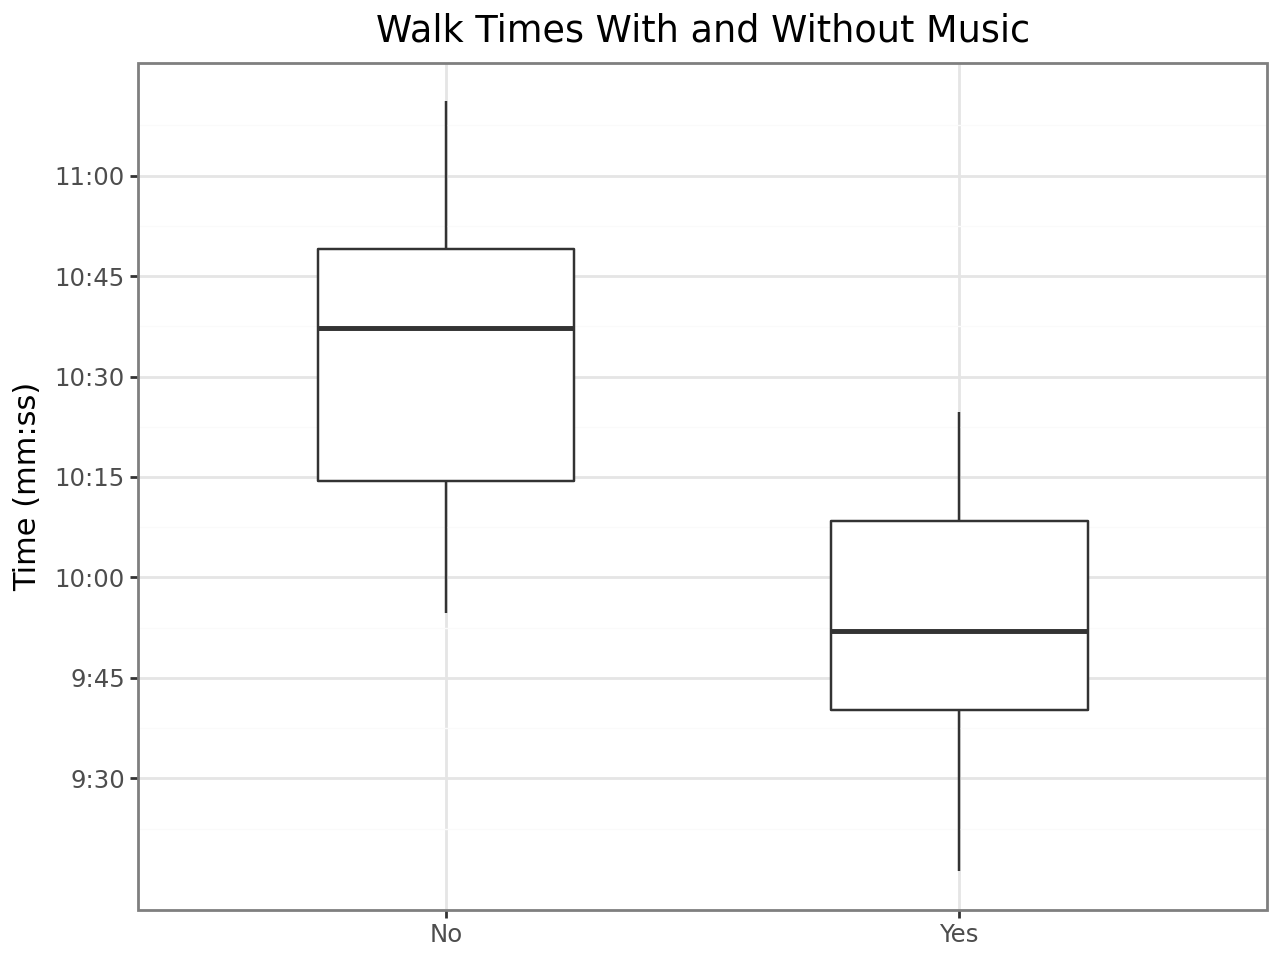
\includegraphics[
    width=\linewidth,
    height=.25\textheight,
    keepaspectratio]
    {box_and_whisker_plot.png}
  \caption{Box‐and‐whisker plot of walk times.}
  \label{fig:walkbox}
\end{figure}


I alternated between music and non-music days instead of doing all the 'music' walks first and the 'no music' walks later. Twenty straight trips without music would have been a miserable experience for me, but the bigger problem was the weather. I started collecting this data in the winter and finished in the spring. I didn't want the weather to have an effect on the data collection. I think I would walk slower in the winter months regardless of whether I am listening to music or not (maybe a project for next year). I would be less comfortable, and heavier clothing would weigh me down. By switching back and forth each day, both conditions—music and no music—were exposed to about the same mix of winter and spring weather. That keeps any seasonal slowdown from biasing the comparison.

\section{Methodology}
Let's turn to hypothesis testing to see if there’s convincing evidence that I walk faster with music than without. Let $\theta_m$ be the true mean walking time (in seconds) when listening to music, and let $\theta_{nm}$ be the true mean walking time when not listening. Formally, at $\alpha = 0.01$, we'll test
\[
\begin{array}{rlcrl}
H_0:\; & \theta_m \ge \theta_{nm}
        & \multirow{2}{*}{\quad\text{vs.}\quad}
        & H_A:\; & \theta_m < \theta_{nm} \\[0.5ex]
       & \theta_m - \theta_{nm} \ge 0 
        & 
        &        & \theta_m - \theta_{nm} < 0
\end{array}
\]
After analyzing my data, I haven't seen any signs of non-normality. There are no outliers, and by the \textit{Central Limit Theorem}, even 20 samples will yield a roughly Gaussian distribution of the mean. Moreover, Welch’s t-test is known to be robust to mild departures from normality, especially when there are no extreme outliers.

Because the population variance $\sigma^2$ is unknown and our sample sizes are modest $(n<30)$, a z-test isn’t appropriate. Instead, we employ a two-sample t-test, which uses the sample variances in its standard‐error term. 


Since we're running a t-test, we need the degree of freedom $\nu$ to get the exact distribution. Our variances are unequal, so instead of $\nu = n_1 +n_2 -2$, we have to use Welch's formula: 
\begin{equation*}
\begin{split}
    \nu & = \frac{(\frac{s_m^2}{n_m}+\frac{s_{nm}^2}{n_{nm}})^2}{\frac{(s_m^2/n_m)^2}{n_m - 1}+\frac{(s_{nm}^2/n_{nm})^2}{n_{nm}-1}} \\ \\
    & = \frac{(\frac{17.60^2}{20}+ \frac{21.48^2}{20})^2}{\frac{(17.60^2 / 20)^2}{20-1}+\frac{(21.48^2 / 20)^2}{20-1}} \\ \\
    & = \frac{1486.68}{40.68} \\ \\
   \nu &  \approx 37
\end{split}
\end{equation*}

Like any parametric test, we need to compute a test statistic:

\begin{equation*}
\begin{split}
    \hat{\hat{t}} & = \frac{\bar{X}_m - \bar{X}_{nm}}{\sqrt{\frac{s^2_m}{n_m} - \frac{s^2_{nm}}{n_{nm}}}} \\ \\
    & = \frac{593.93 - 633.19}{\sqrt{\frac{17.60^2}{20}+ \frac{21.48^2}{20}}} \\ \\
    & = \frac{-39.26}{6.21} \\ \\
    \hat{\hat{t}} & = -6.32
\end{split}
\end{equation*}

\section{Running the Test}
To decide whether or not we retain $H_0$,  we have to check whether our observed test statistic lies in the retainment region for a one-sided t-test at $\alpha = 0.01$. With $\nu = 37$, the retainment region for $T_{0.01, 37}$ is $[-2.43, \infty)$. Our test statistic of $\hat{\hat{t}} = -6.32$ does not fall into this region, and we consequently reject $H_0$ that I don't walk faster while listening to music. \\ \\
Alternatively, let's also compute the p-value. If it is greater than $\alpha = 0.01$ then we can retain $H_0$, otherwise we reject it. 
\begin{equation*}
\begin{split}
    \hat{\hat{p}} &= \mathbb{P}(T_\nu \leq \hat{\hat{t}}) \\ \\
    \hat{\hat{p}} & = \mathbb{P}(T_{37} \leq -6.32) \\ \\
    \hat{\hat{p}} & = 1.2 \times 10^{-7}
\end{split}
\end{equation*} \\
The p-value is much lower than $\alpha = 0.01$ so as expected, we reject $H_0$.


\section{Bootstrapping}
Let's say we don't want to assume my walk follow any form of normality. Fortunately, there are a number of non-parametric methods we can use to test my hypothesis. One of these methods is \textit{Bootstrapping}. 
We will generate $B = 10,000$ replicates by resampling with replacement separately from the "music" and "no music" groups. For each new \textit{b}, I compute \\ \\
\[
\Delta ^{(b)} = \bar{X}^{(b)} _m - \bar{X}^{(b)} _{nm}
\textrm{ (where $\Delta^{(b)}$ is an entry in our new Bootstrapped dataset)}
\] \\
From this distribution, the 99 percentile interval is [-59.4, -20.8] seconds, which excludes zero by a lot. In the accompanying histogram, the dashed red lines mark the 0.5\% and the 99.5\% quantiles. Because the entire interval lies well below 0, we confidentally reject
\[
H_0: \theta_m - \theta_{nm} \geq 0 \textrm{ in favor of } H_a: \theta_m - \theta_{nm} < 0, 
\] 
providing a fully data-driven confirmation that I walk significantly faster while listening to music.

\begin{figure}[H]
  \centering
  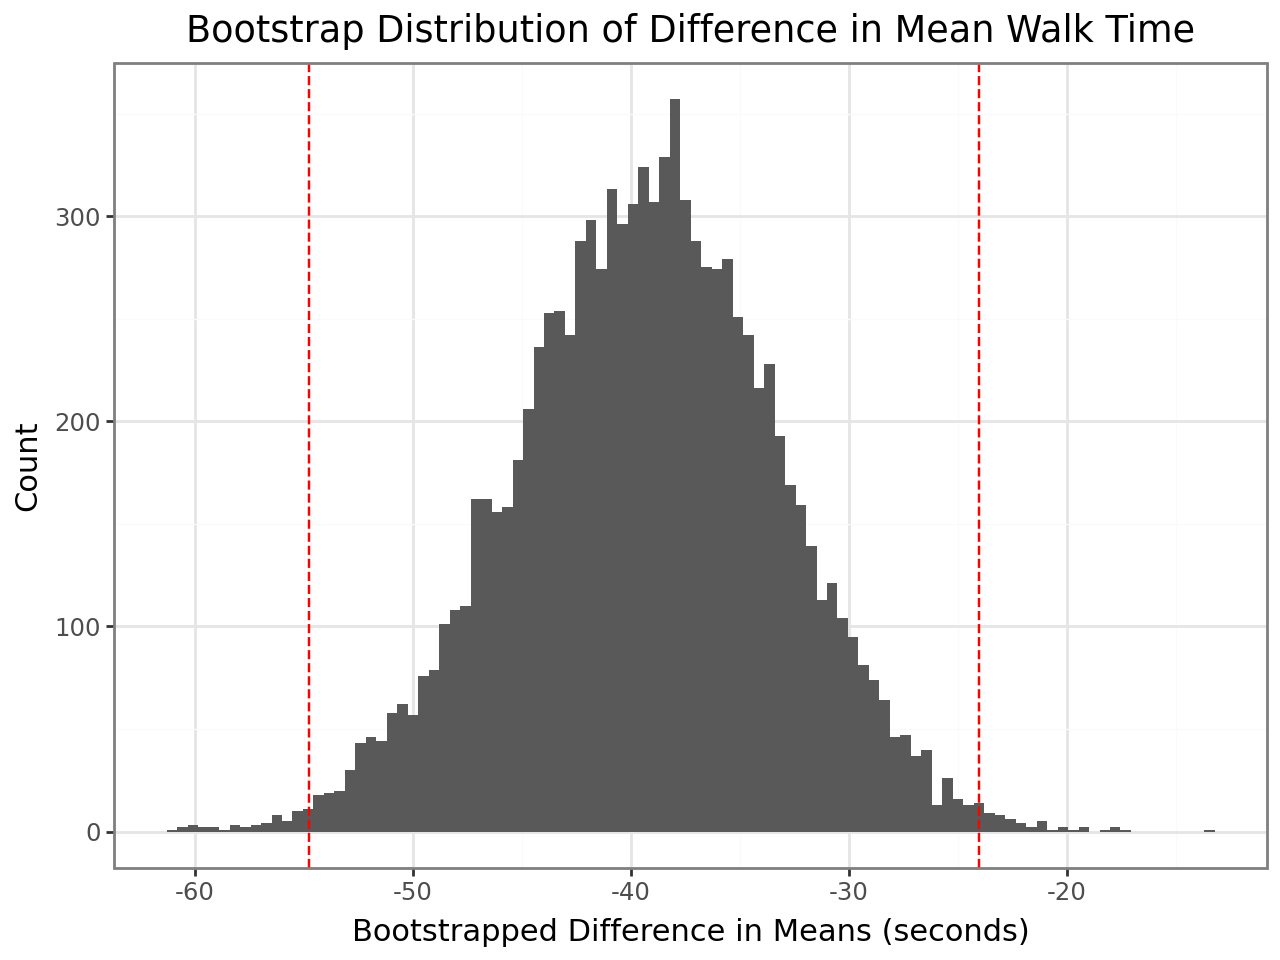
\includegraphics[
    width=\linewidth,
    height=.40\textheight,
    keepaspectratio]
    {bootstrapped_distribution.png}
  \caption{Bootstrapped Distribution of Difference of Mean Walk Times.}
  \label{fig:walkbox}
\end{figure}

\section{Conclusion}
To summarize, across 40 walks the average walking time with music was 594 seconds (9:54) versus 633 seconds (10:33) without music - a 40 second improvment! A Welch two-sample t-test, and a 99\% Bootstrapped percentile interval both reject $H_0$ at $\alpha = 0.01$. Therefore, I can conclude with high confidence that listening to music significantly speeds up my walking speed.

\end{document}

